\setcounter{chapter}{0}

\part{Data Technology}

\chapter{Dataset}
\sections{data_technology/dataset}

\chapter{Data Quality}
\label{chap:data-quality}
Abbiamo sottoposto i dataset ad un processo di analisi finalizzato 
all'esplorazione dei dati e all'incremento della loro qualità. In particolare, 
data la natura dei dati e il nostro scopo, siamo ricorsi alle dimensioni di 
completezza, consistenza e leggibilità.

% Metriche dei dataset analizzati singolarmente

\section{Completezza}
\sections{data_technology/completezza}

\section{Consistenza di chiave}
\sections{data_technology/consistenza}

\section{Leggibilità}
\sections{data_technology/leggibilita}

\section{Acquisizione di nuovi dati}
% FIXME

\chapter{Data Integration}
\label{chap:data-integration}

%deduplication
\section{Deduplication}
\sections{data_technology/deduplicazione}

% record linkage
\section{Record Linkage}
\label{sec:record-linkage}
\sections{data_technology/record_linkage}

%fusion
\section{Data Fusion}
\sections{data_technology/data_fusion}

\chapter{Analisi di almeno 2 dimensioni di qualità e relative metriche delle features successivamente utilizzate}

\chapter{Analisi descrittive dei dati integrati}

\begin{figure}[htb]
	\centering
	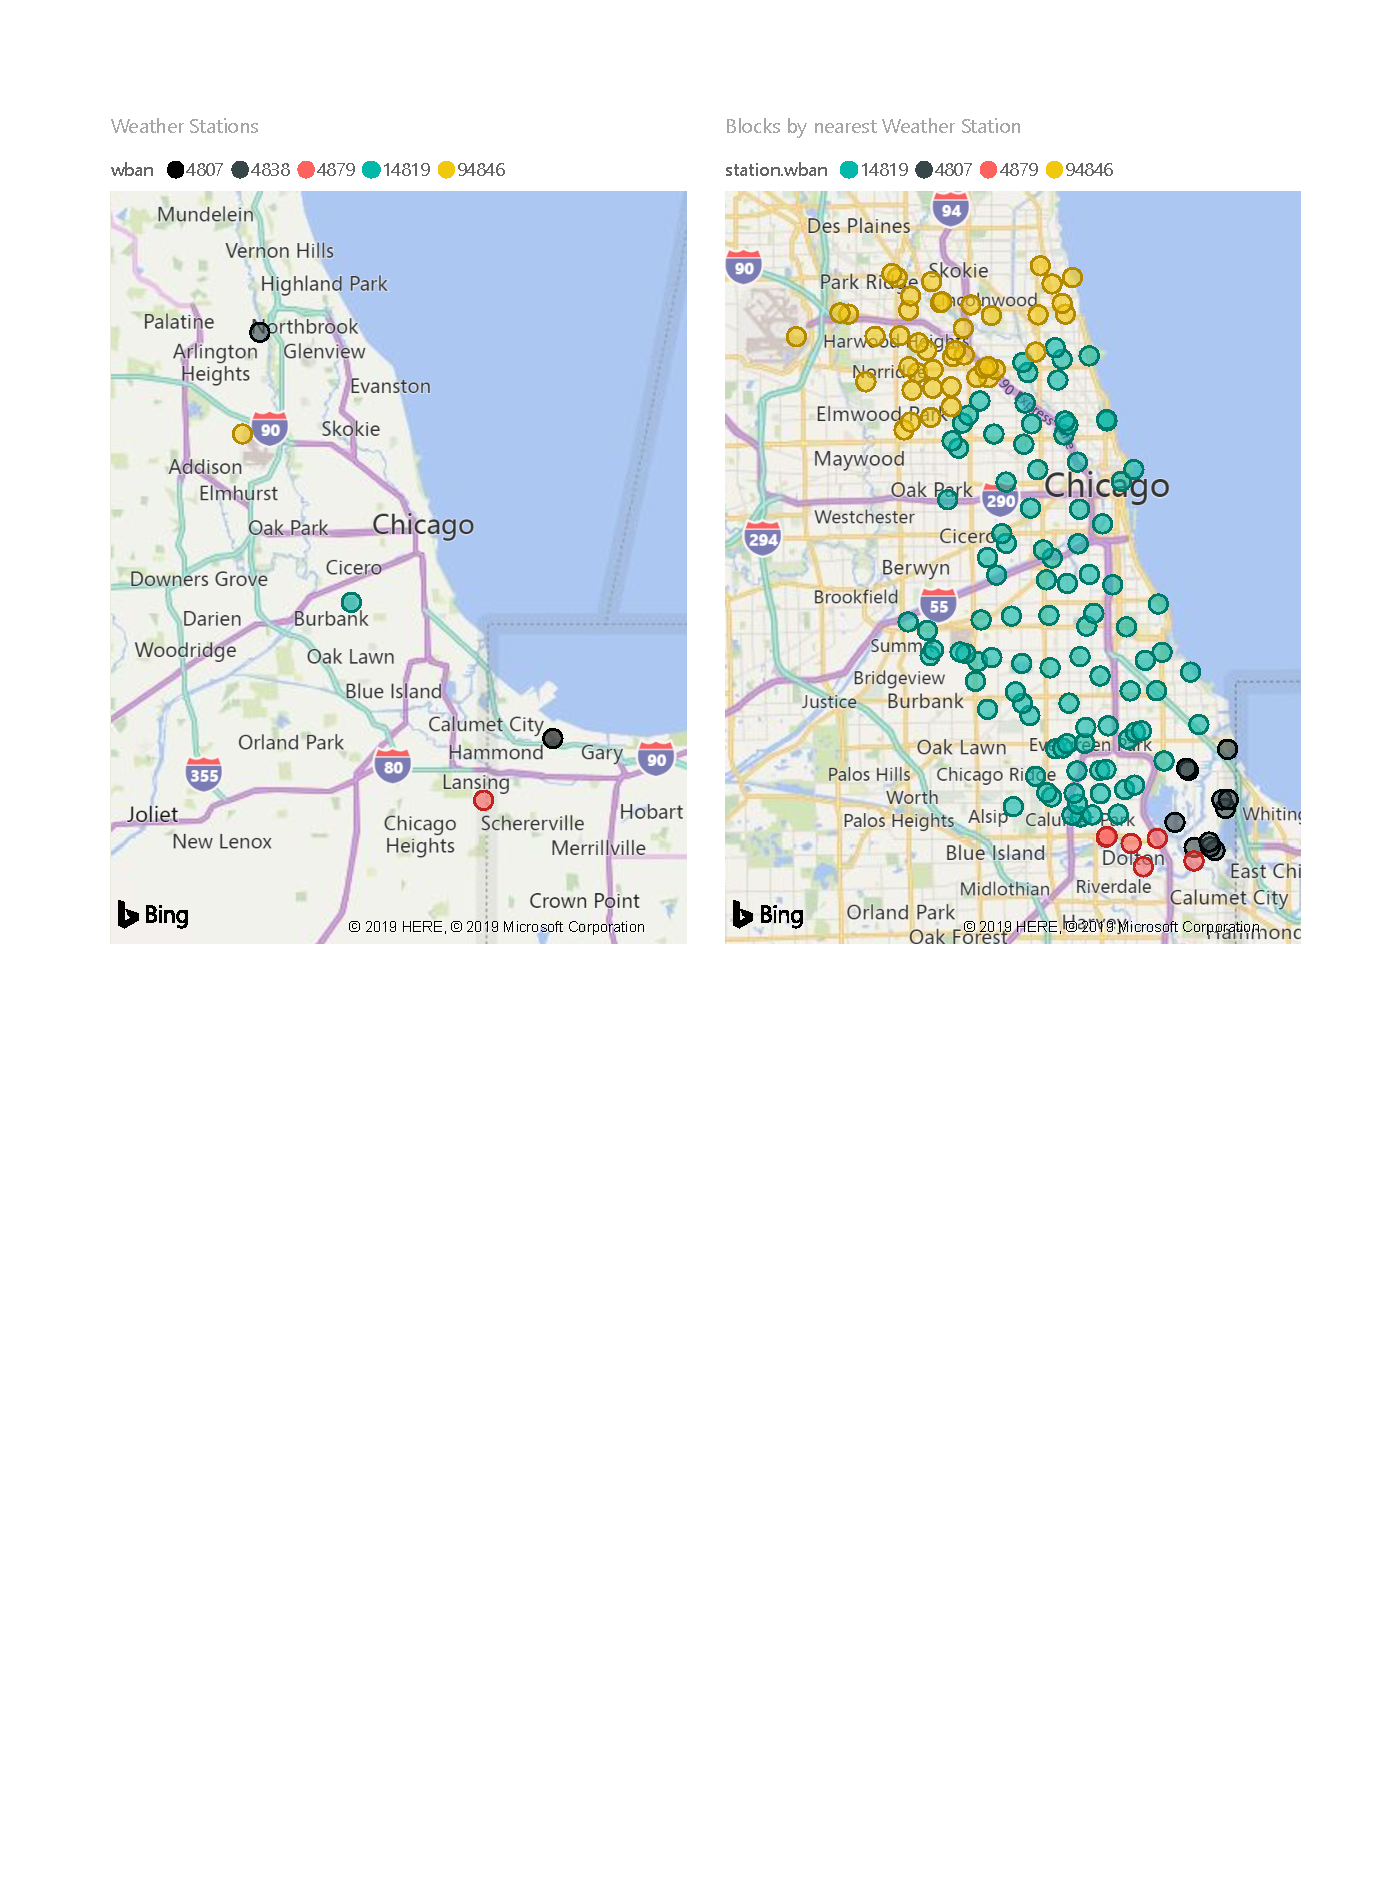
\includegraphics[width=0.4\columnwidth]{images/WeatherStations}
	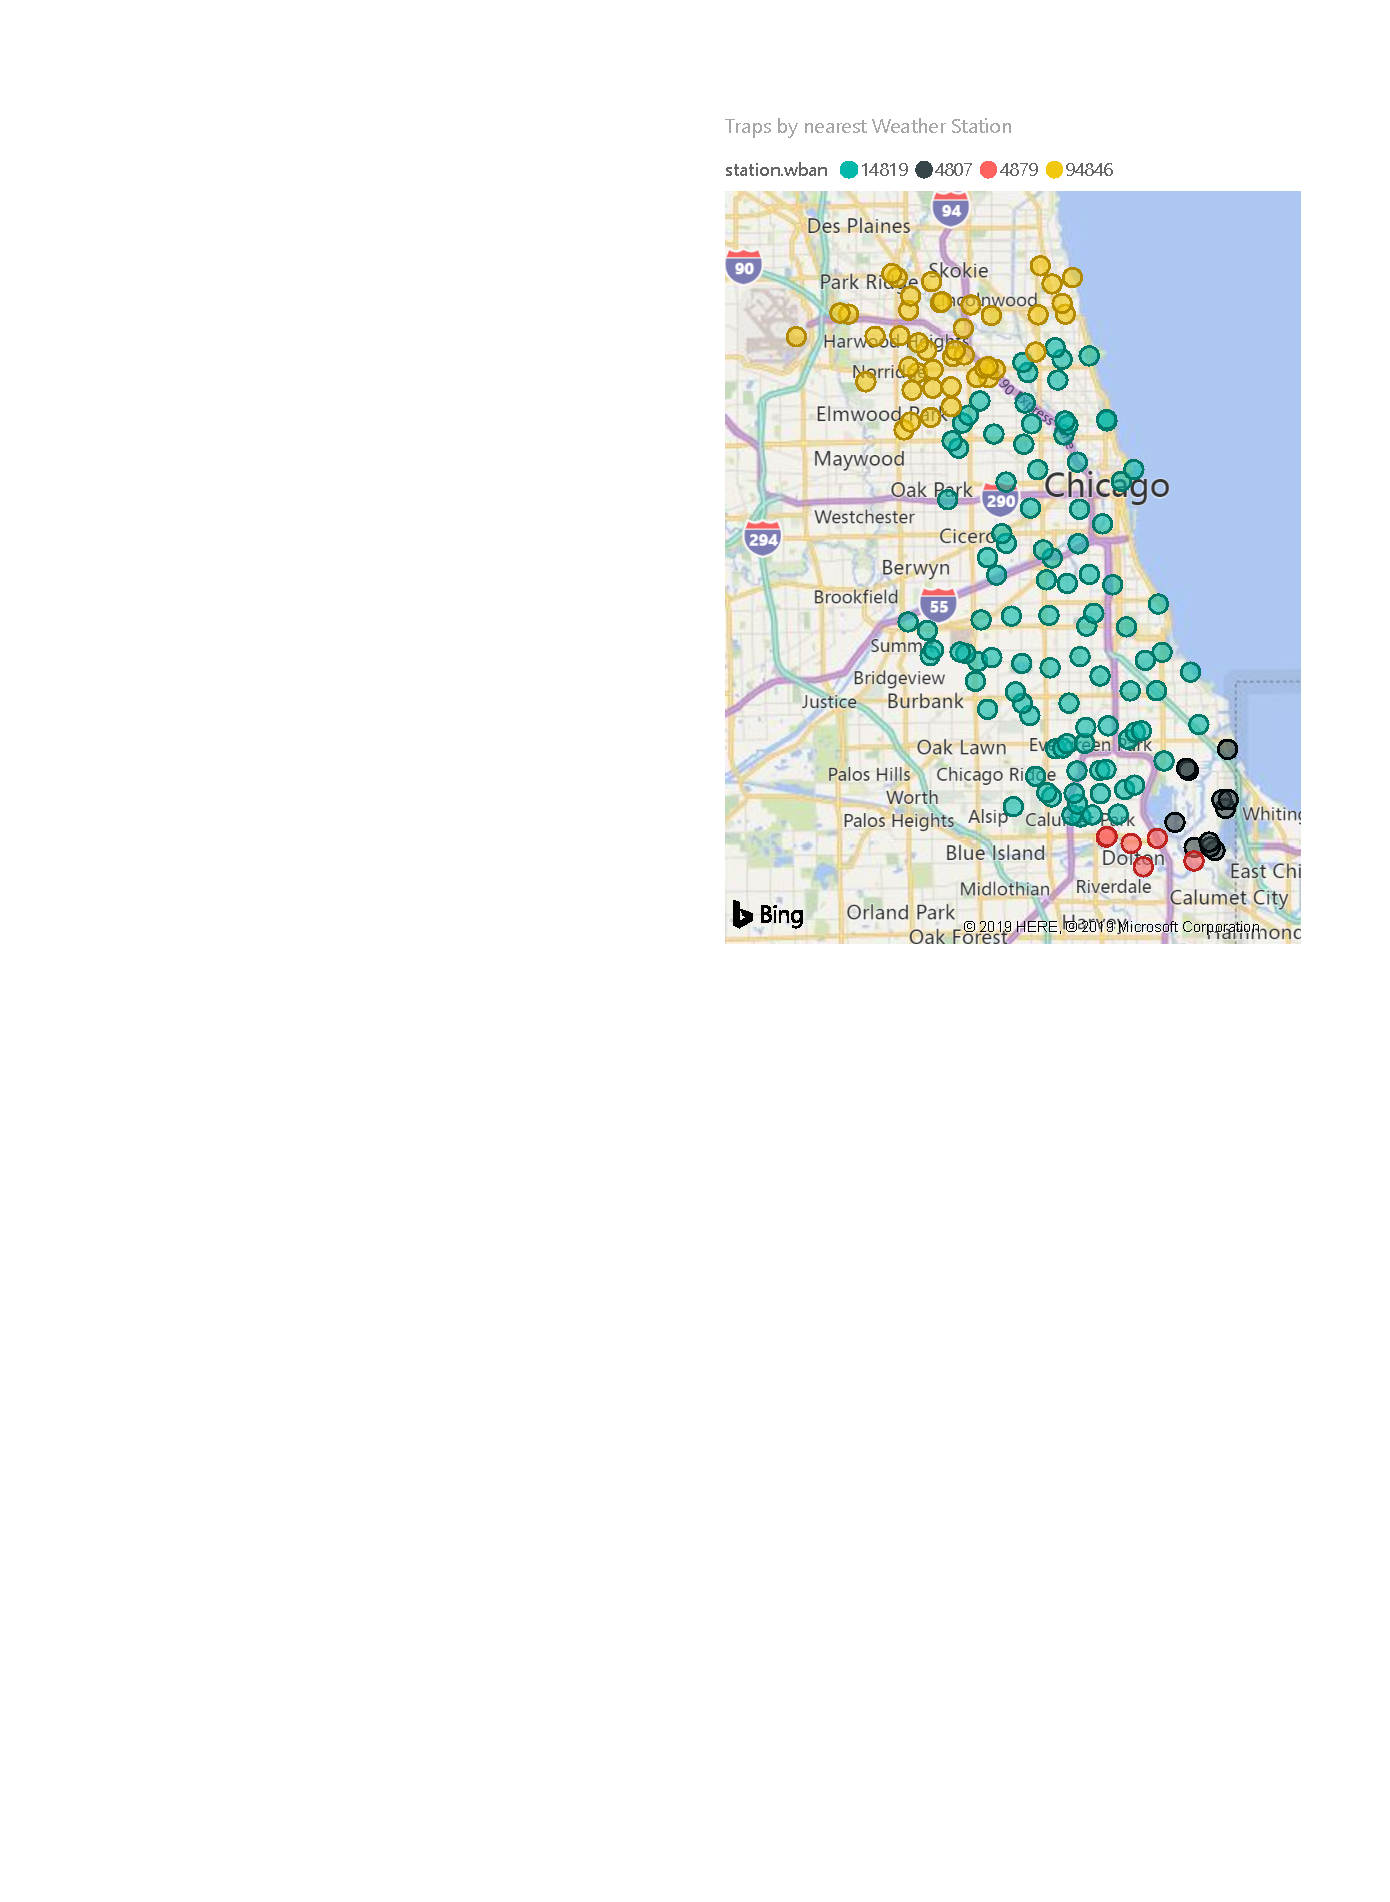
\includegraphics[width=0.4\columnwidth]{images/TrapsByNN}
	\caption{FIXME Visualizzazione dei 64 filtri convoluzionali appresi dal 
	layer \textbf{conv1} della rete ResNet-34. Il blu scuro rappresenta i 
	valori negativi, il verde quelli prossimi allo zero e il giallo quelli 
	positivi}
	\label{fig:weather-stations}
\end{figure}
